\documentclass[screen, aspectratio=169]{beamer}
\usepackage[T1]{fontenc}
%\usepackage[utf8]{inputenc}

% Use the NTNU-temaet for beamer 
% \usetheme[style=ntnu|simple|vertical|horizontal, 
%     language=bm|nn|en, 
%     smalltitle, 
%     city=all|trondheim|alesund|gjovik]{ntnu2017}
\usetheme[style=ntnu,language=en]{ntnu2017}

\usepackage[english]{babel}
\usepackage[style=numeric,backend=biber,natbib=false,sorting=none]{biblatex}

\title[HCI-intro]{Human Computer Interaction}
\subtitle{NIMEs (focus on evaluation and practices)}
\author[A. Xamb{\'o}]{Anna Xamb{\'o}}
\institute[NTNU]{Department of Music, NTNU}
\date{29 October 2019}
%\date{} % To have an empty date

\addbibresource{../hci-lectures.bib} % Add bibliography database

% Set the reference style to numeric.
% See here: http://tex.stackexchange.com/questions/68080/beamer-bibliography-icon
\setbeamertemplate{bibliography item}[text] 

% Set bibliography fonts to a small size.
\renewcommand*{\bibfont}{\footnotesize}

\begin{document}

\begin{frame}
  \titlepage
\end{frame}

% Alternatively, special title page command to get a different background
% \ntnutitlepage
\begin{frame}
\frametitle{Comments on the 1st week}
\begin{itemize}
\item HCI Individual Assignment Day 1
\item HCI Group Assignment Day 1
\item HCI Individual Assignment Day 2
\item HCI Group Assignment Day 2 \dots
\end{itemize}
\end{frame}
%
\begin{frame}
\frametitle{Learning Outcomes}
\begin{itemize}
\item Get a sense of the synergies between HCI and NIME research.
\item Explore a range of key practices in the NIME community from an HCI perspective (focusing on evaluation).
\item Identify the NIME practices relevant to personal projects.
\item Discern the format of NIME paper writing.
\end{itemize}
\end{frame}
%
\begin{frame}
\frametitle{Class Structure}
\begin{itemize}
\item 10.15-10.20 Comments on the 1st week.
\item 10.20-10.50 Mapping the NIME field: Evaluation at NIME.
\item 10.50-11.00 Selection of papers.
\item 11.00-11.30 Teamwork: Understanding NIME paper writing.
\item 11.30-12.00 The teams summarize to the group their selected paper (5--7 min per group). 
%\item 10.40-11.00 Presentation/lecture of CSCM.
\end{itemize}
\end{frame}
%
\begin{frame}
\frametitle{}
\Huge{Evaluation @ NIME}
\end{frame}
%
\begin{frame}
\frametitle{Preparation: Reading}
\begin{itemize}
\item Send a summary (1 page max.) of the following article:
\begin{itemize}
\item Jeronimo Barbosa, Joseph Malloch, Marcelo Wanderley, and St\'{e}phane Huot. 2015. What does `Evaluation' mean for the NIME community? \emph{Proceedings of the International Conference on New Interfaces for Musical Expression}, Louisiana State University, pp. 156--161. \cite{Barbosa.et.al.2015.evaluationNIME}\\
\end{itemize}
The summary should include: the research question, the approach used to address the research question, the main findings, and the main contribution.
\end{itemize}
\end{frame}
%
\begin{frame}
\frametitle{Warm-up Activity: Evaluation @ NIME}
 \begin{figure}
	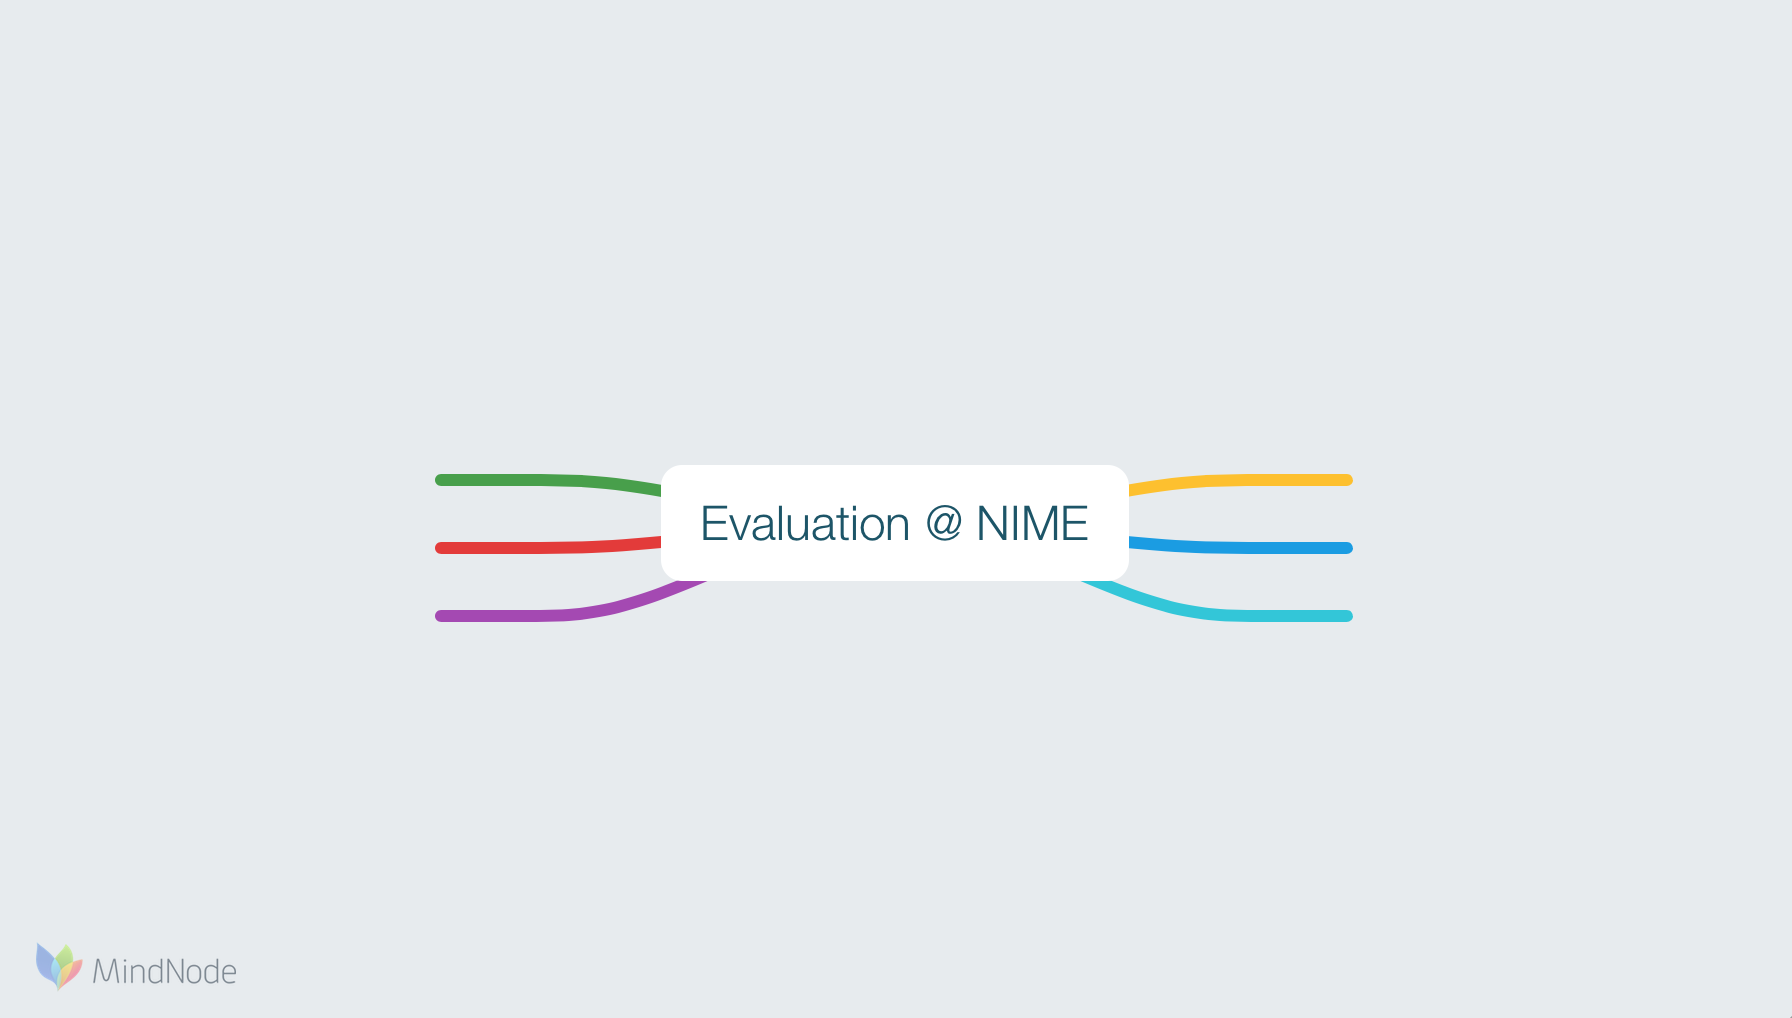
\includegraphics[scale=0.35]{img/mindmap-eval-nime.png}
    \end{figure}	
\end{frame}
%
\begin{frame}
\frametitle{}
\begin{figure}
	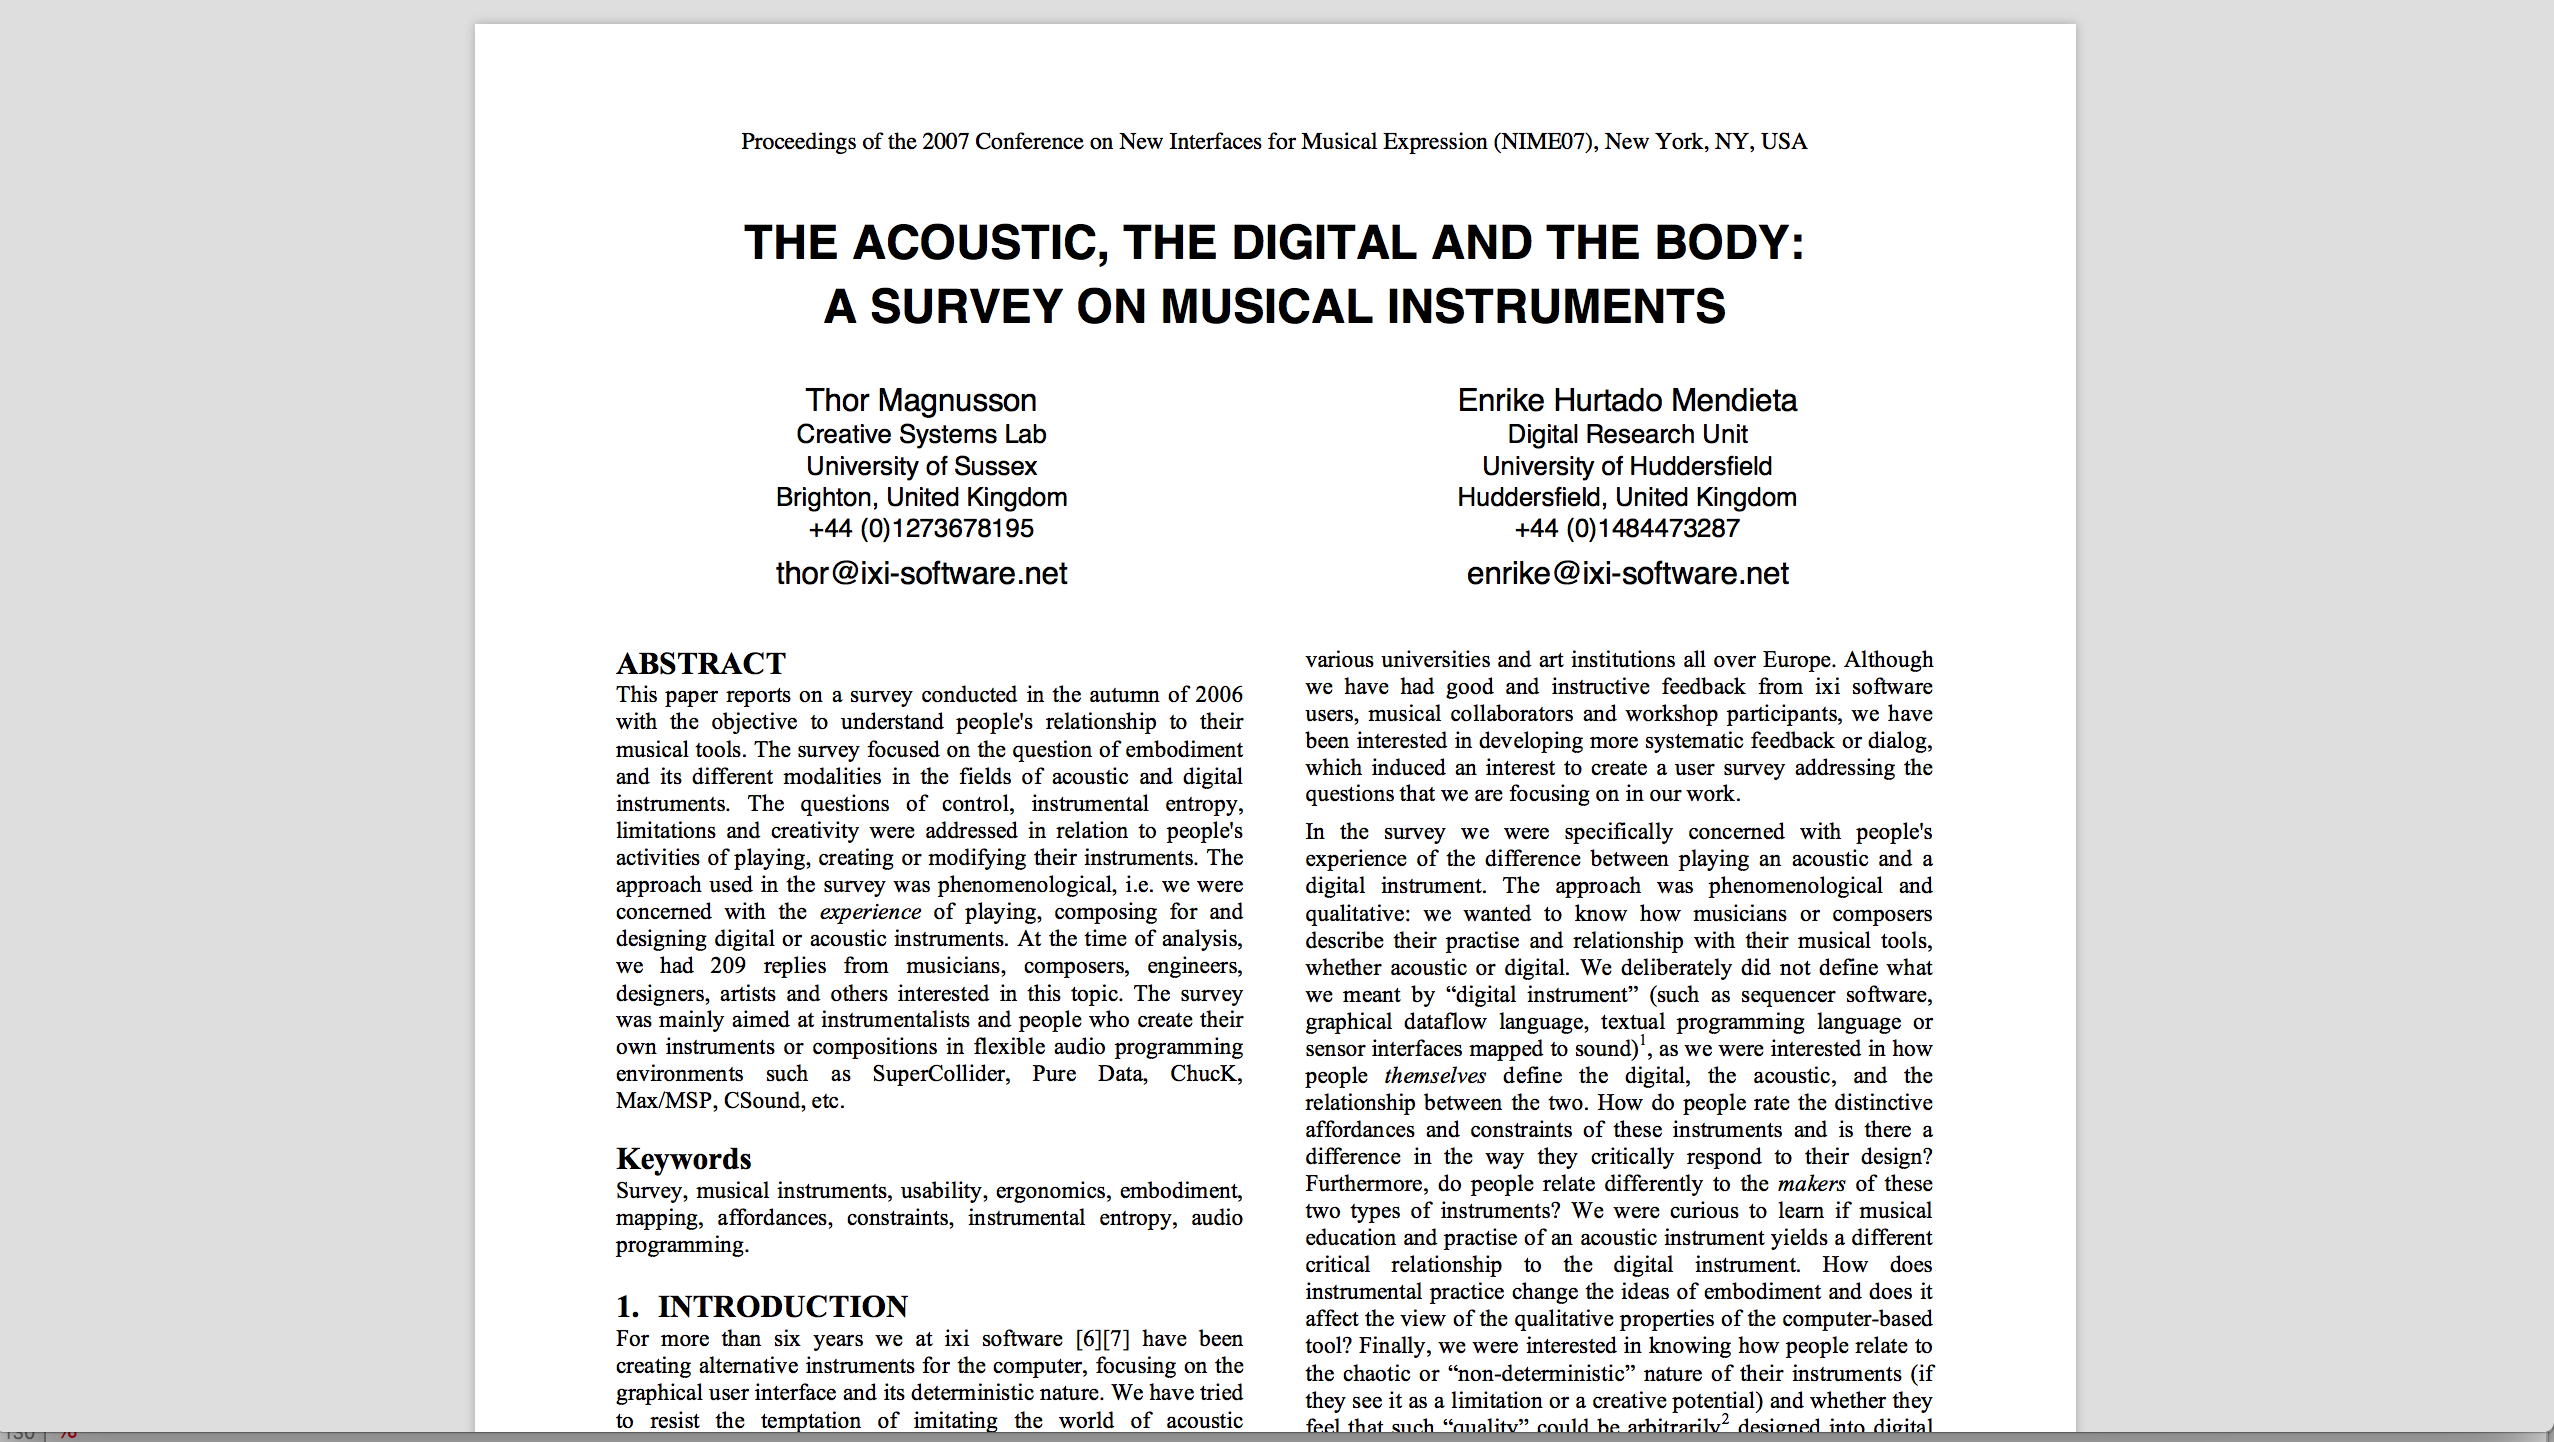
\includegraphics[scale=0.31]{img/Magnusson-Mendieta-2007.png}\\
	    \cite{Magnusson.Mendieta.2007.NIME}\\
    \end{figure}		
\end{frame}
%
\begin{frame}
\frametitle{The Acoustic, The Digital and the Body}
\begin{itemize}
\item RQ: Understand people's relationship to their musical tools focusing on the question of embodiment and its different modalities in the fields of acoustic and digital instruments.
\item Evaluation:
\begin{itemize}
\item 209 replies from musicians, composers, engineers, designers, artists.
\item Quantitative and qualitative questions.
\end{itemize}
\item 5 main themes:
\begin{itemize}
\item  Acoustic vs\ digital instruments.
\item Affordances and constraints.
\item The instrument maker criticised.
\item Entropy and control ininstruments.
\item Time and embodiment.
\end{itemize}
\item Contribution: Informs future design and evaluation of musical tools.
\end{itemize}
\end{frame}
%
\begin{frame}
\frametitle{}	
\begin{figure}
	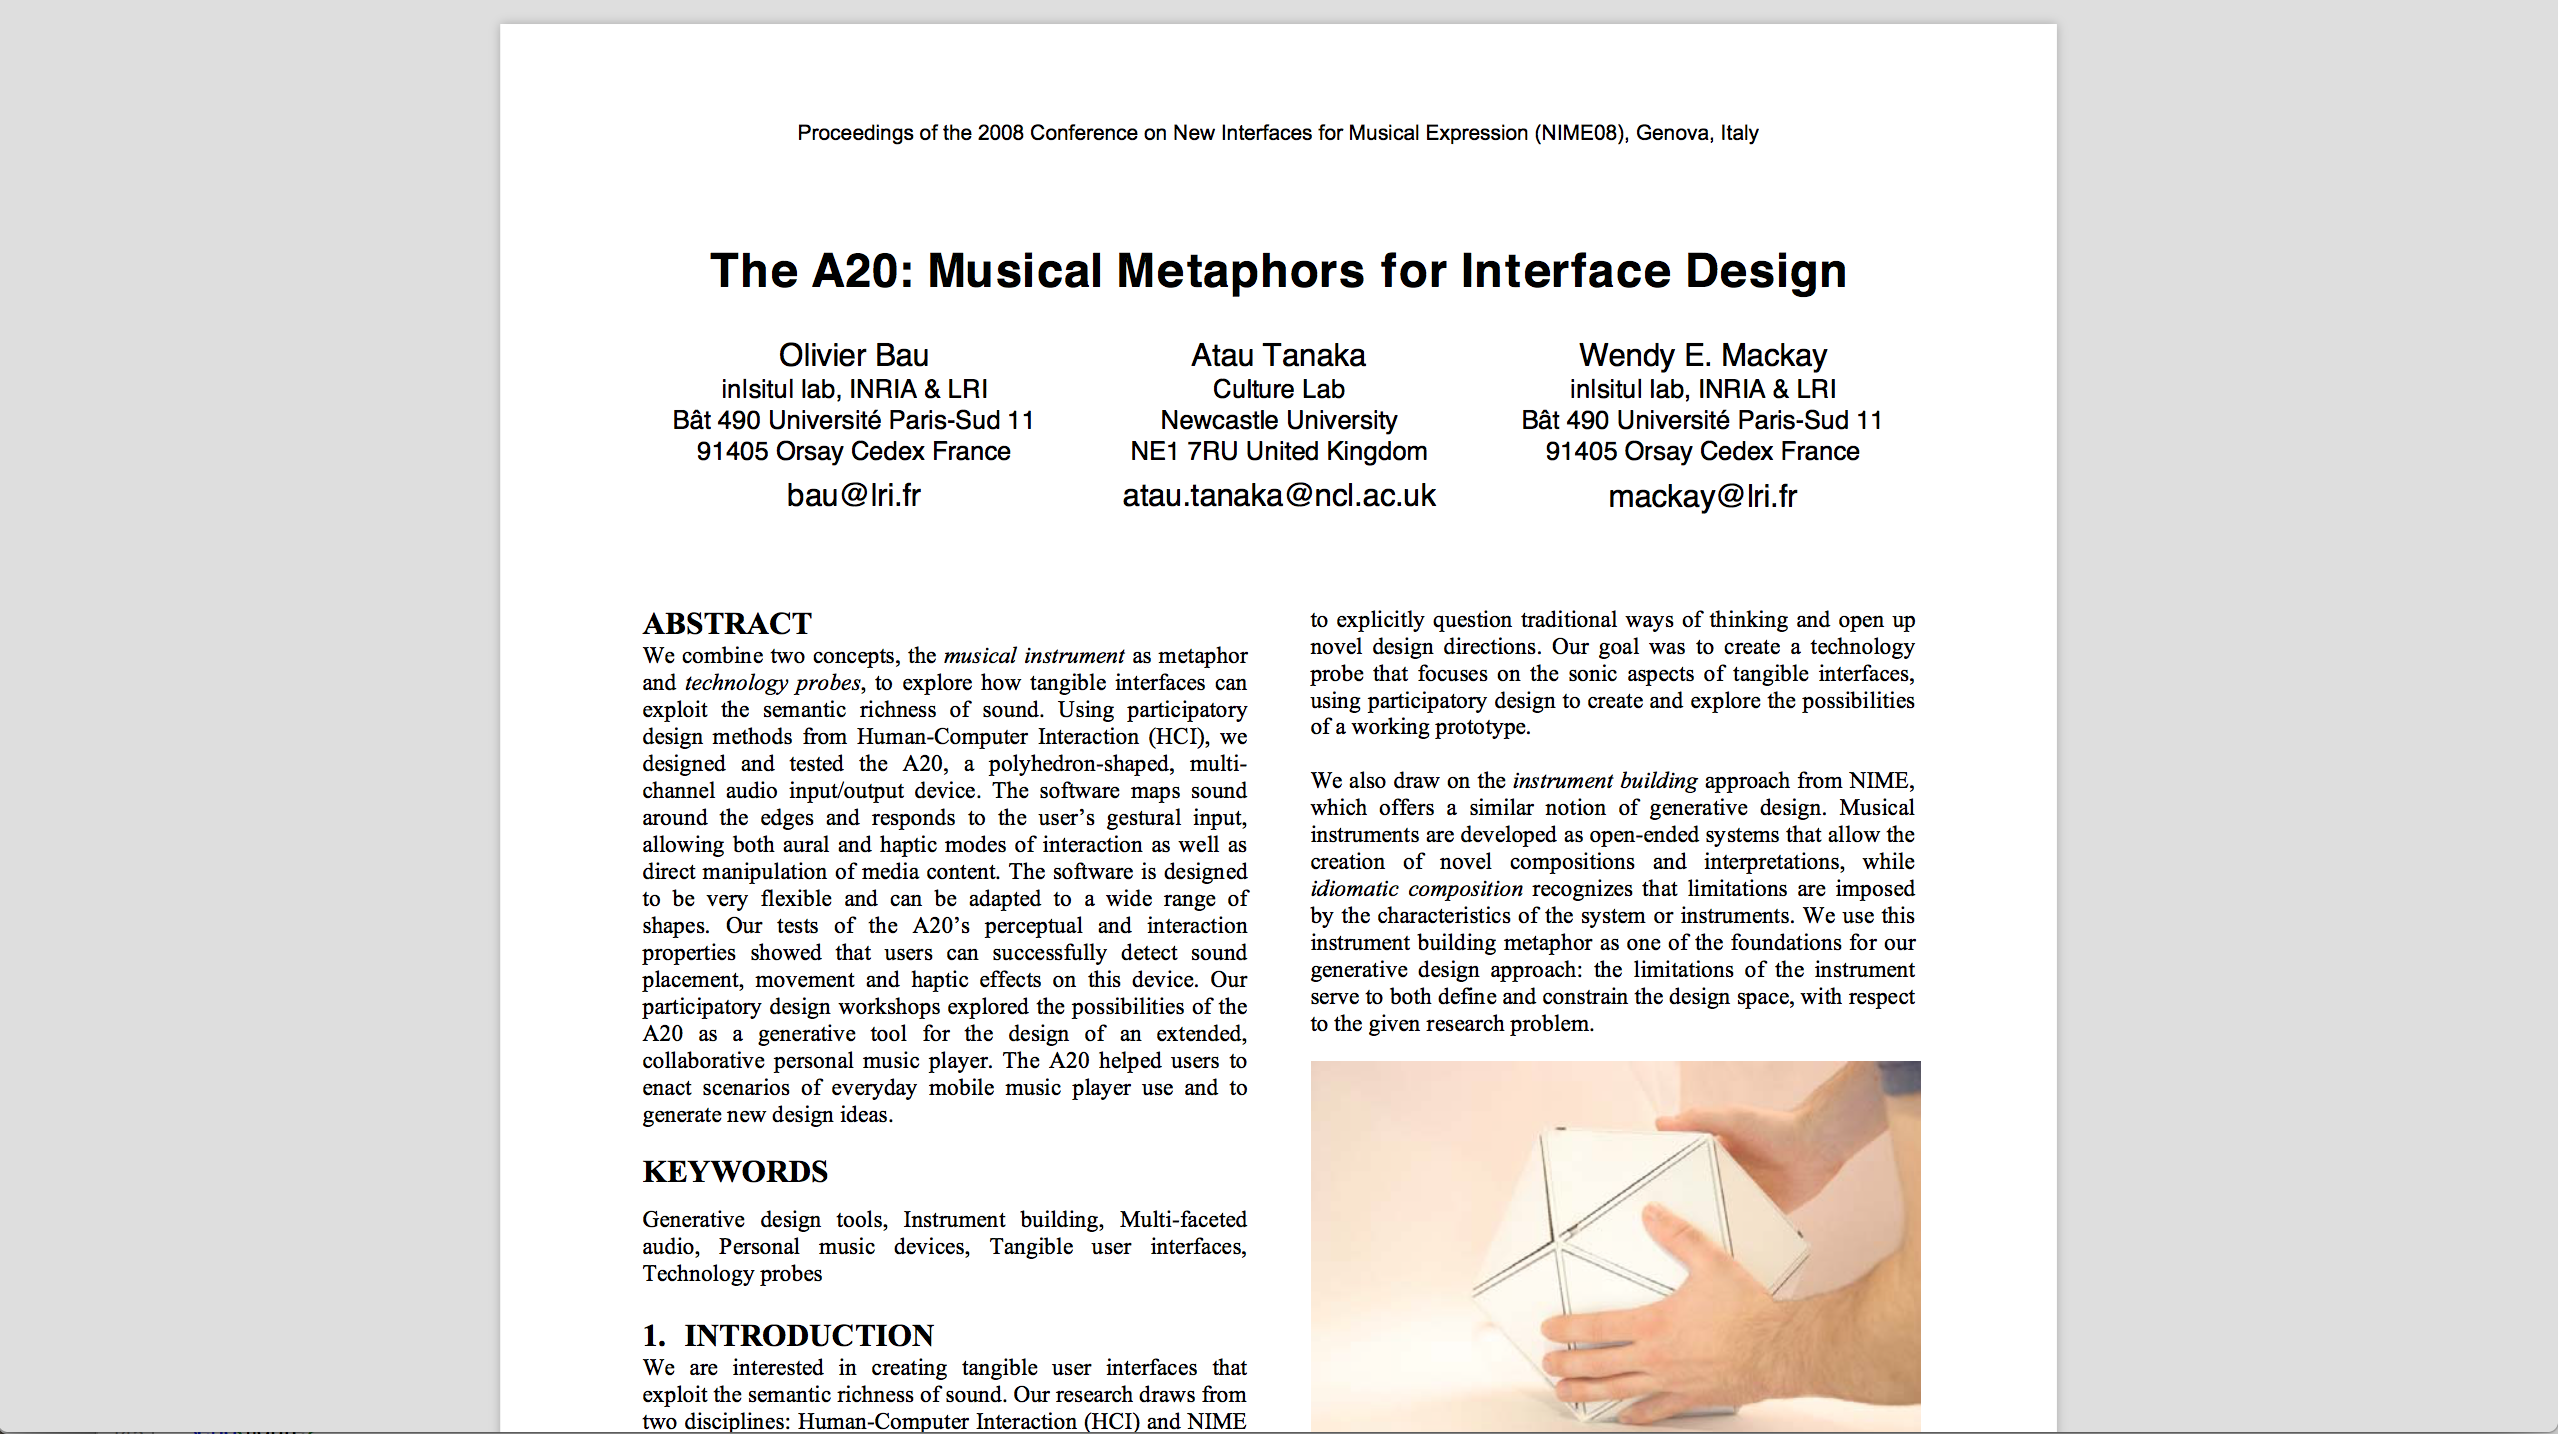
\includegraphics[scale=0.29]{img/Bau-et-al-2008.png}\\
	    \cite{Bau.et.al.2008.NIME}\\
	       {\scriptsize  \url{http://www.olivierbau.com/a20.php}}
    \end{figure}	
\end{frame}
%
\begin{frame}
\frametitle{Musical Metaphors for Interface Design}	
\begin{itemize}
\item RQ: Exploration of how tangible interfaces can exploit the semantic richness of sound.
\item Evaluation:
\begin{itemize}
\item Evaluation of a polyhedron-shaped, multi- channel audio input/output device with participatory design methods from HCI (16 participants).
\item Evaluation 1: Focus on the perceptual characteristics of the device.
\item Evaluation 2: cultural probes / technology probes, participatory workshops with tasks and a design theme.
\end{itemize}
\item Results: Evidence of a platform for generating and exploring new sound interaction ideas.
\item Contribution: Informs future design and evaluation of tangible interfaces for music and new approaches to sound design.
\end{itemize}
\end{frame}
%
\begin{frame}
\frametitle{}
\begin{figure}
	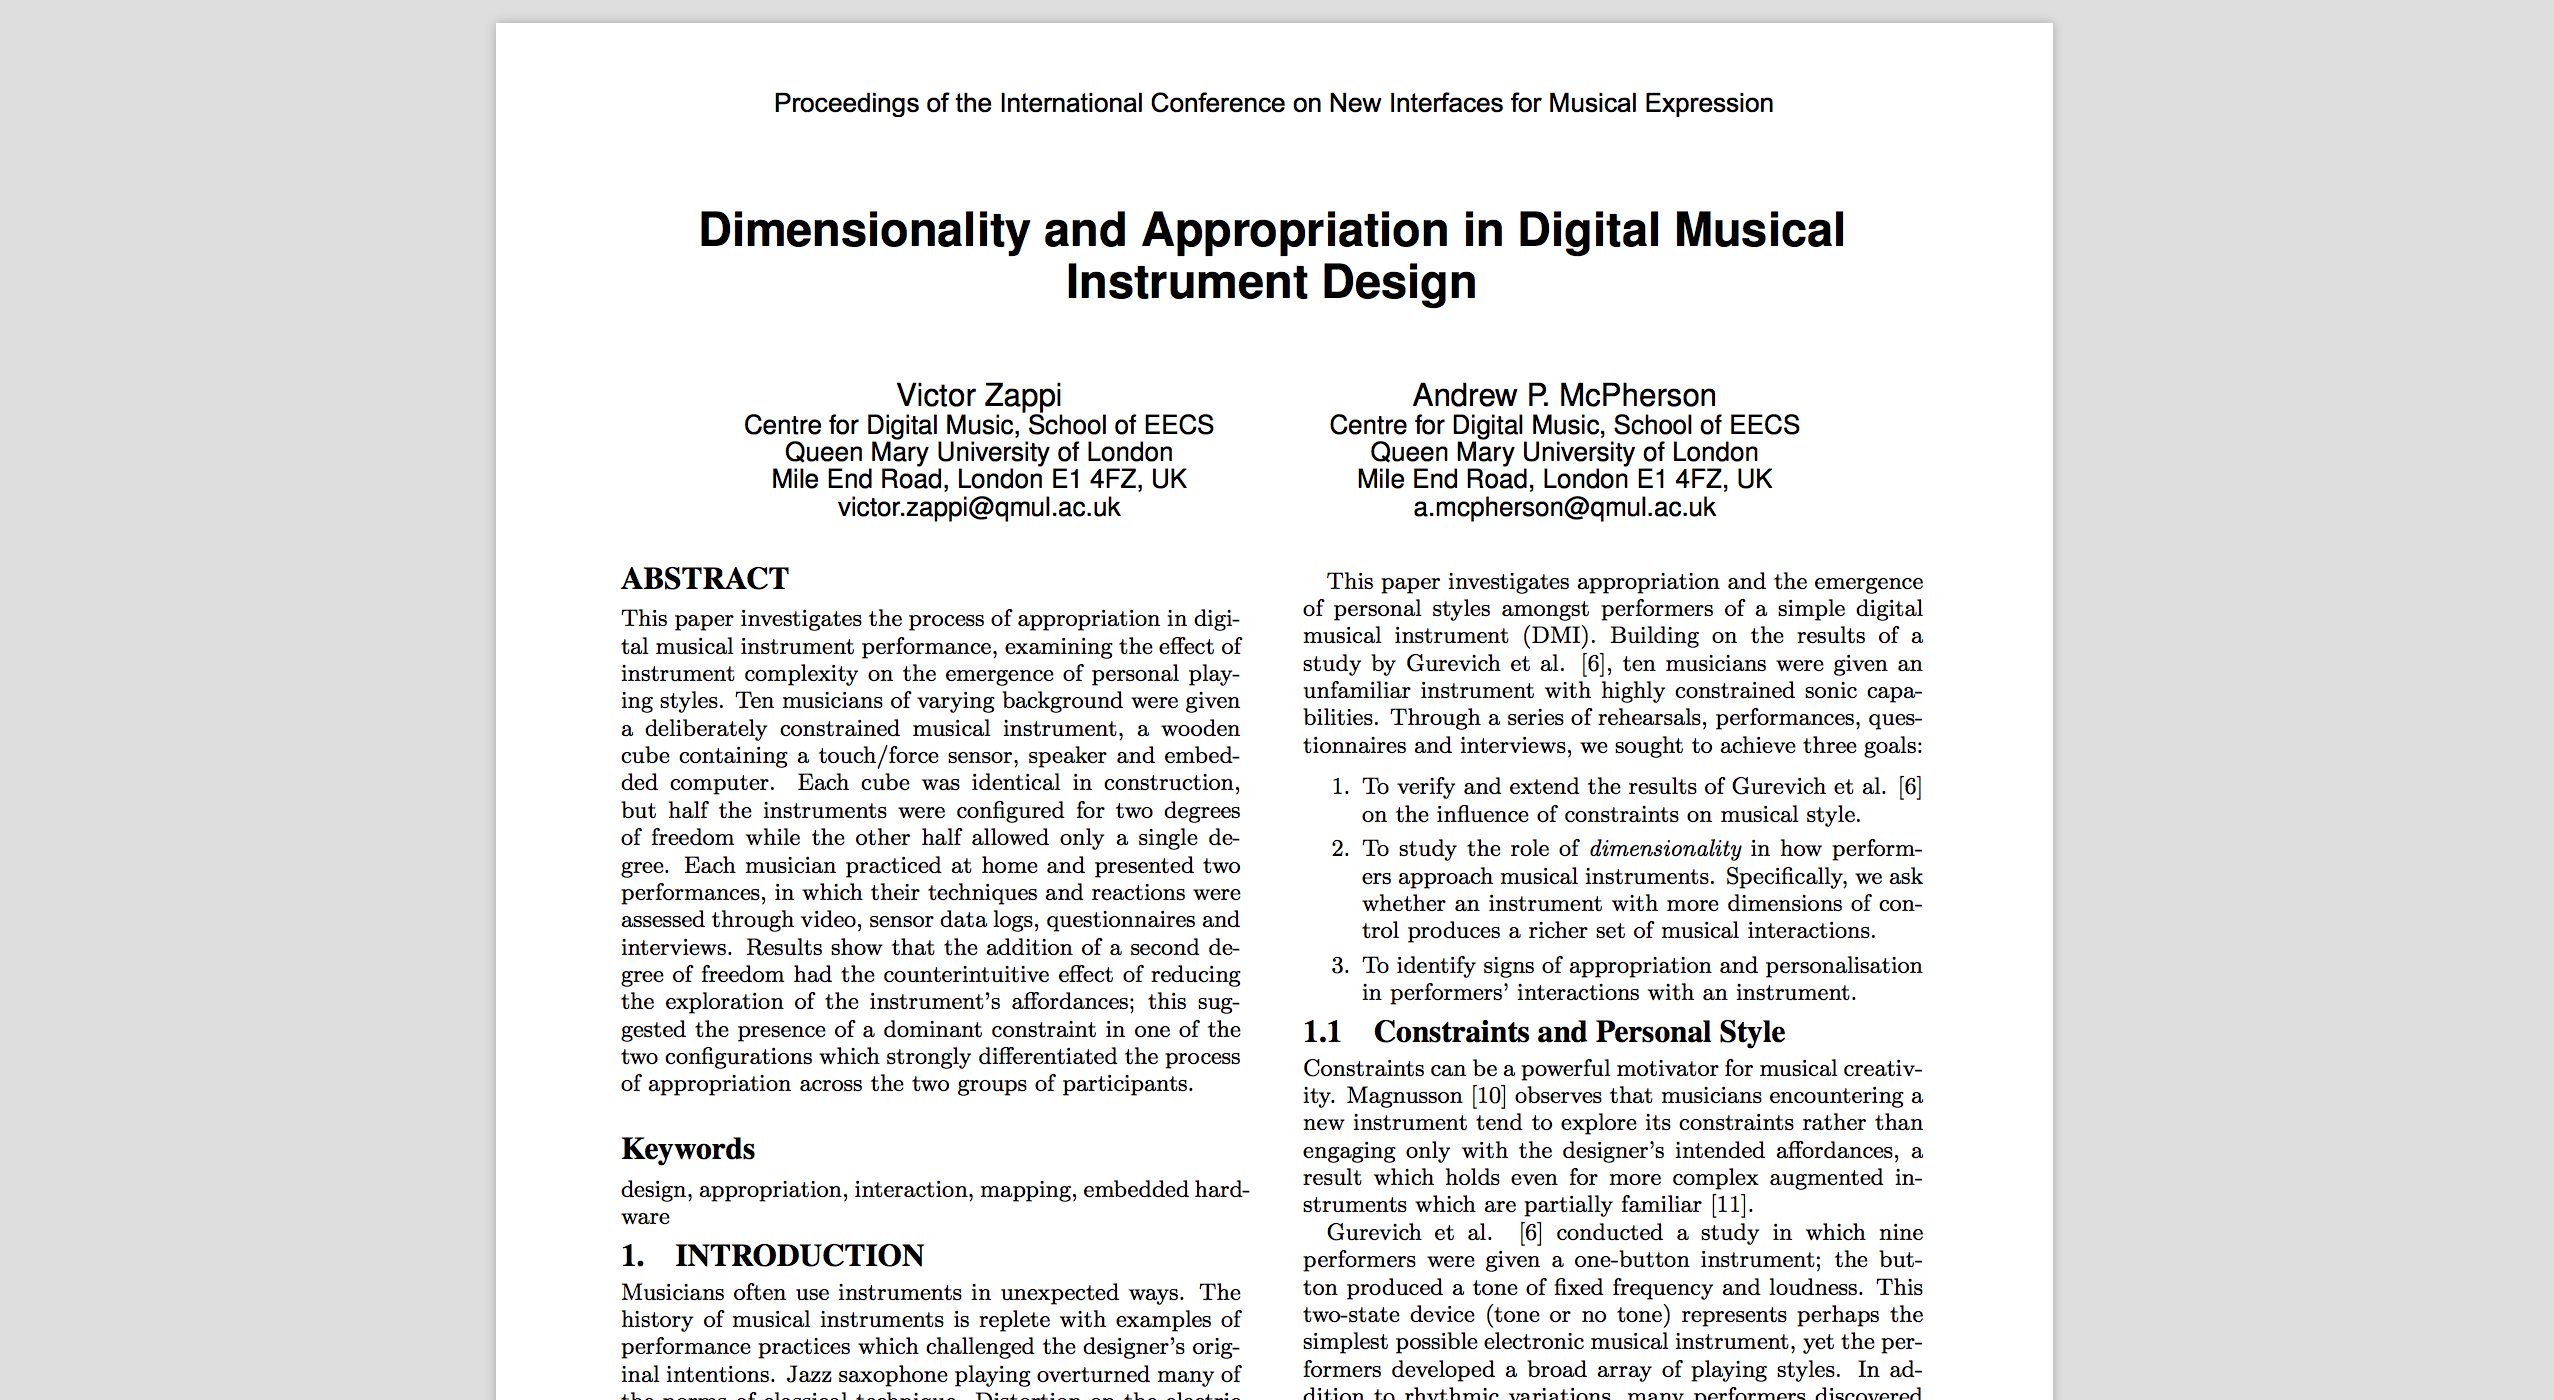
\includegraphics[scale=0.31]{img/Zappi-McPherson-2014.png}\\
	    \cite{Zappi.McPherson.2014.NIME}\\
	       {\scriptsize  \url{http://instrumentslab.org/research/hackable-instruments.html}}
    \end{figure}		
\end{frame}
%
\begin{frame}
\frametitle{Dimensionality and Appropriation (1/2)}	
\begin{figure}
	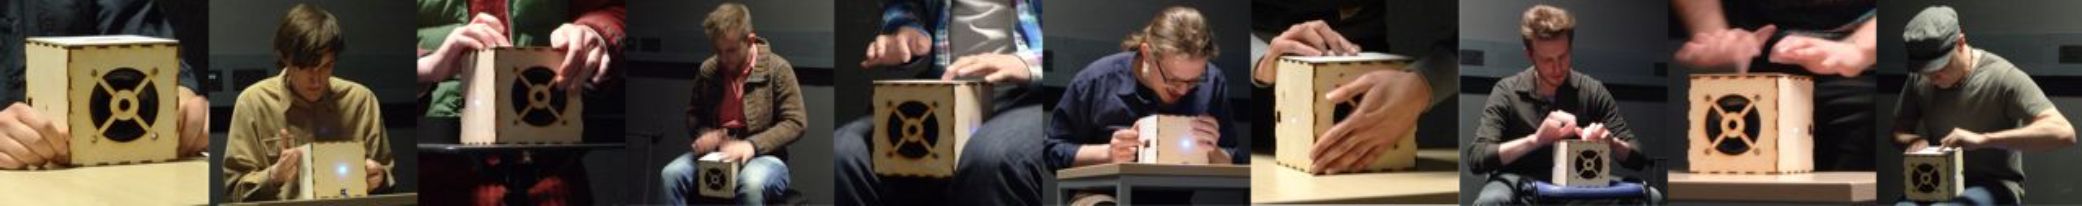
\includegraphics[scale=0.31]{img/Zappi-McPherson-2014-2.png}\\
    \end{figure}	
\begin{itemize}
\item RQ: Investigation of the process of appropriation in digital musical instrument performance, examining the effect of instrument complexity on the emergence of personal playing styles.
\item Evaluation:
\begin{itemize}
\item Ten musicians were given a constrained musical instrument, a wooden cube containing a touch/force sensor, speaker and embedded computer.
\item Half the instruments were configured for two degrees of freedom while the other half allowed only a single degree.
\item Home practice and delivery of 2 performances. Techniques and reactions were assessed through video, sensor data logs, questionnaires and interviews (mixed methods).
\end{itemize}
\end{itemize}
\end{frame}
%
\begin{frame}
\frametitle{Dimensionality and Appropriation (2/2)}	
\begin{figure}
	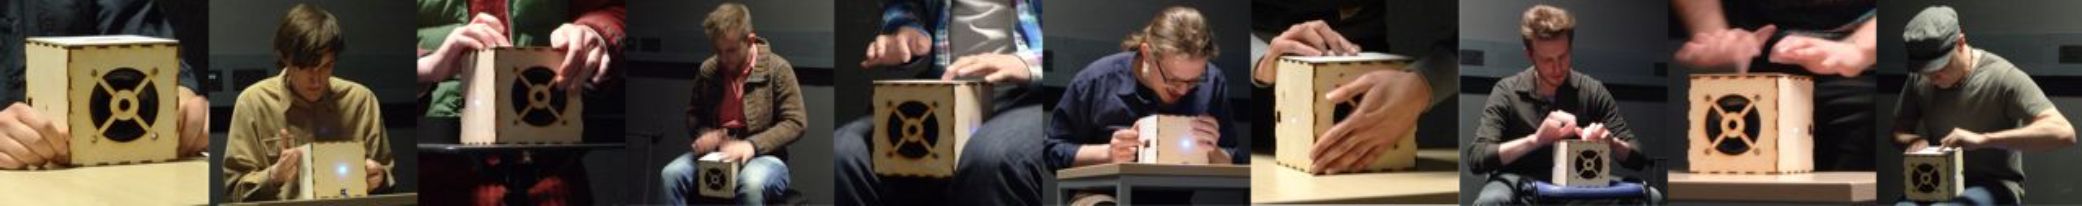
\includegraphics[scale=0.31]{img/Zappi-McPherson-2014-2.png}\\
    \end{figure}	
\begin{itemize}
\item Results: the addition of a second degree of freedom had the counterintuitive effect of reducing the exploration of the instrument's affordances.
\item Contribution: In alignment with the the one-button instrument study \cite{Gurevich.et.al.2010.NIME}. Informs the design of DMIs.
\end{itemize}
\end{frame}%
\begin{frame}
\frametitle{}
\begin{figure}
	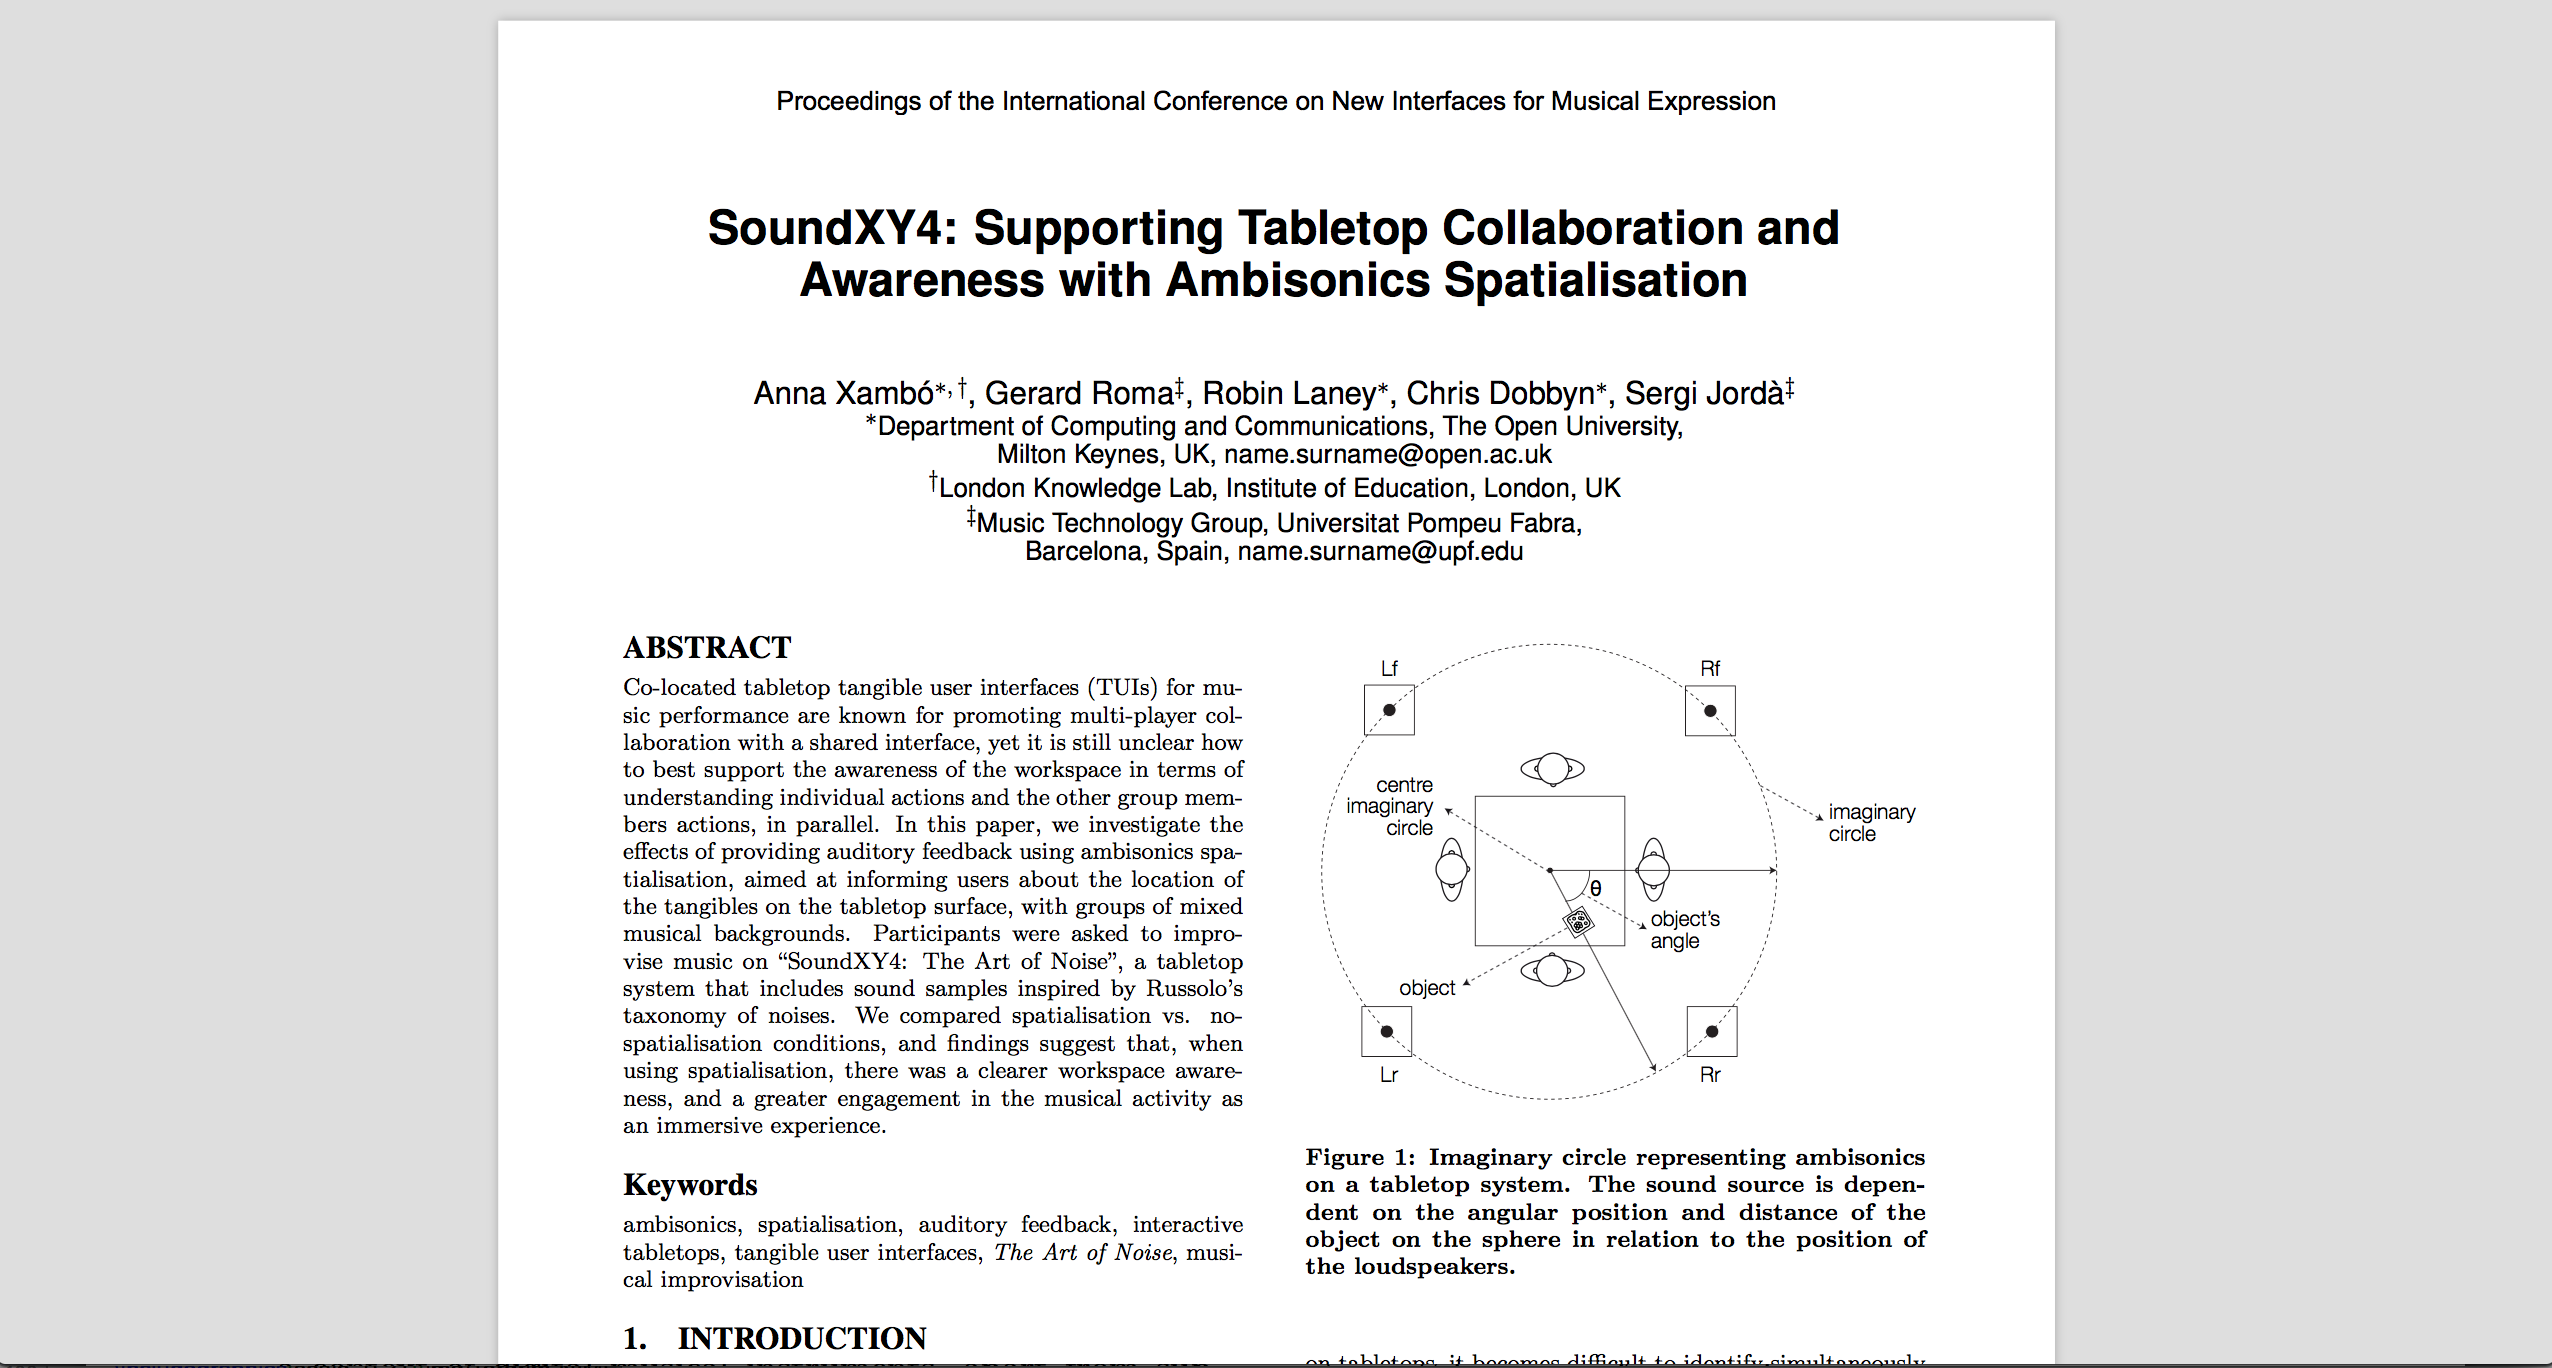
\includegraphics[scale=0.31]{img/Xambo-et-al-2014.png}\\
	    \cite{Xambo.et.al.2014}\\
	    \url{https://vimeo.com/70693984}
    \end{figure}		
\end{frame}
%
\begin{frame}
\frametitle{Supporting Tabletop Collaboration and Awareness}	
\begin{itemize}
\item RQ: How to best support the awareness of the workspace in co-located tabletop tangible user interfaces (TUIs) for music performance. Investigation of the effects of providing auditory feedback using ambisonics spatialisation.
\item Evaluation:
\begin{itemize}
\item Task: Music improvisation in groups of four participants: 8 groups, 32 participants in total.
\item Qualitative analysis (thematic analysis) of video recordings.
\item Themes: Space territoriality; Sounds, categories, and filters; Realistic scenes; Musical immersion.
\item Spatialisation vs.\ no-spatialisation conditions.
\end{itemize}
\item Findings: Spatialization promoted a clearer workspace awareness, and a greater engagement in the musical activity as an immersive experience.
\item Contribution: Informs DMIs design using an ecological approach and the area of computer-supported collaborative work.
\end{itemize}
\end{frame}
%
\begin{frame}
\frametitle{}
 \begin{figure}
	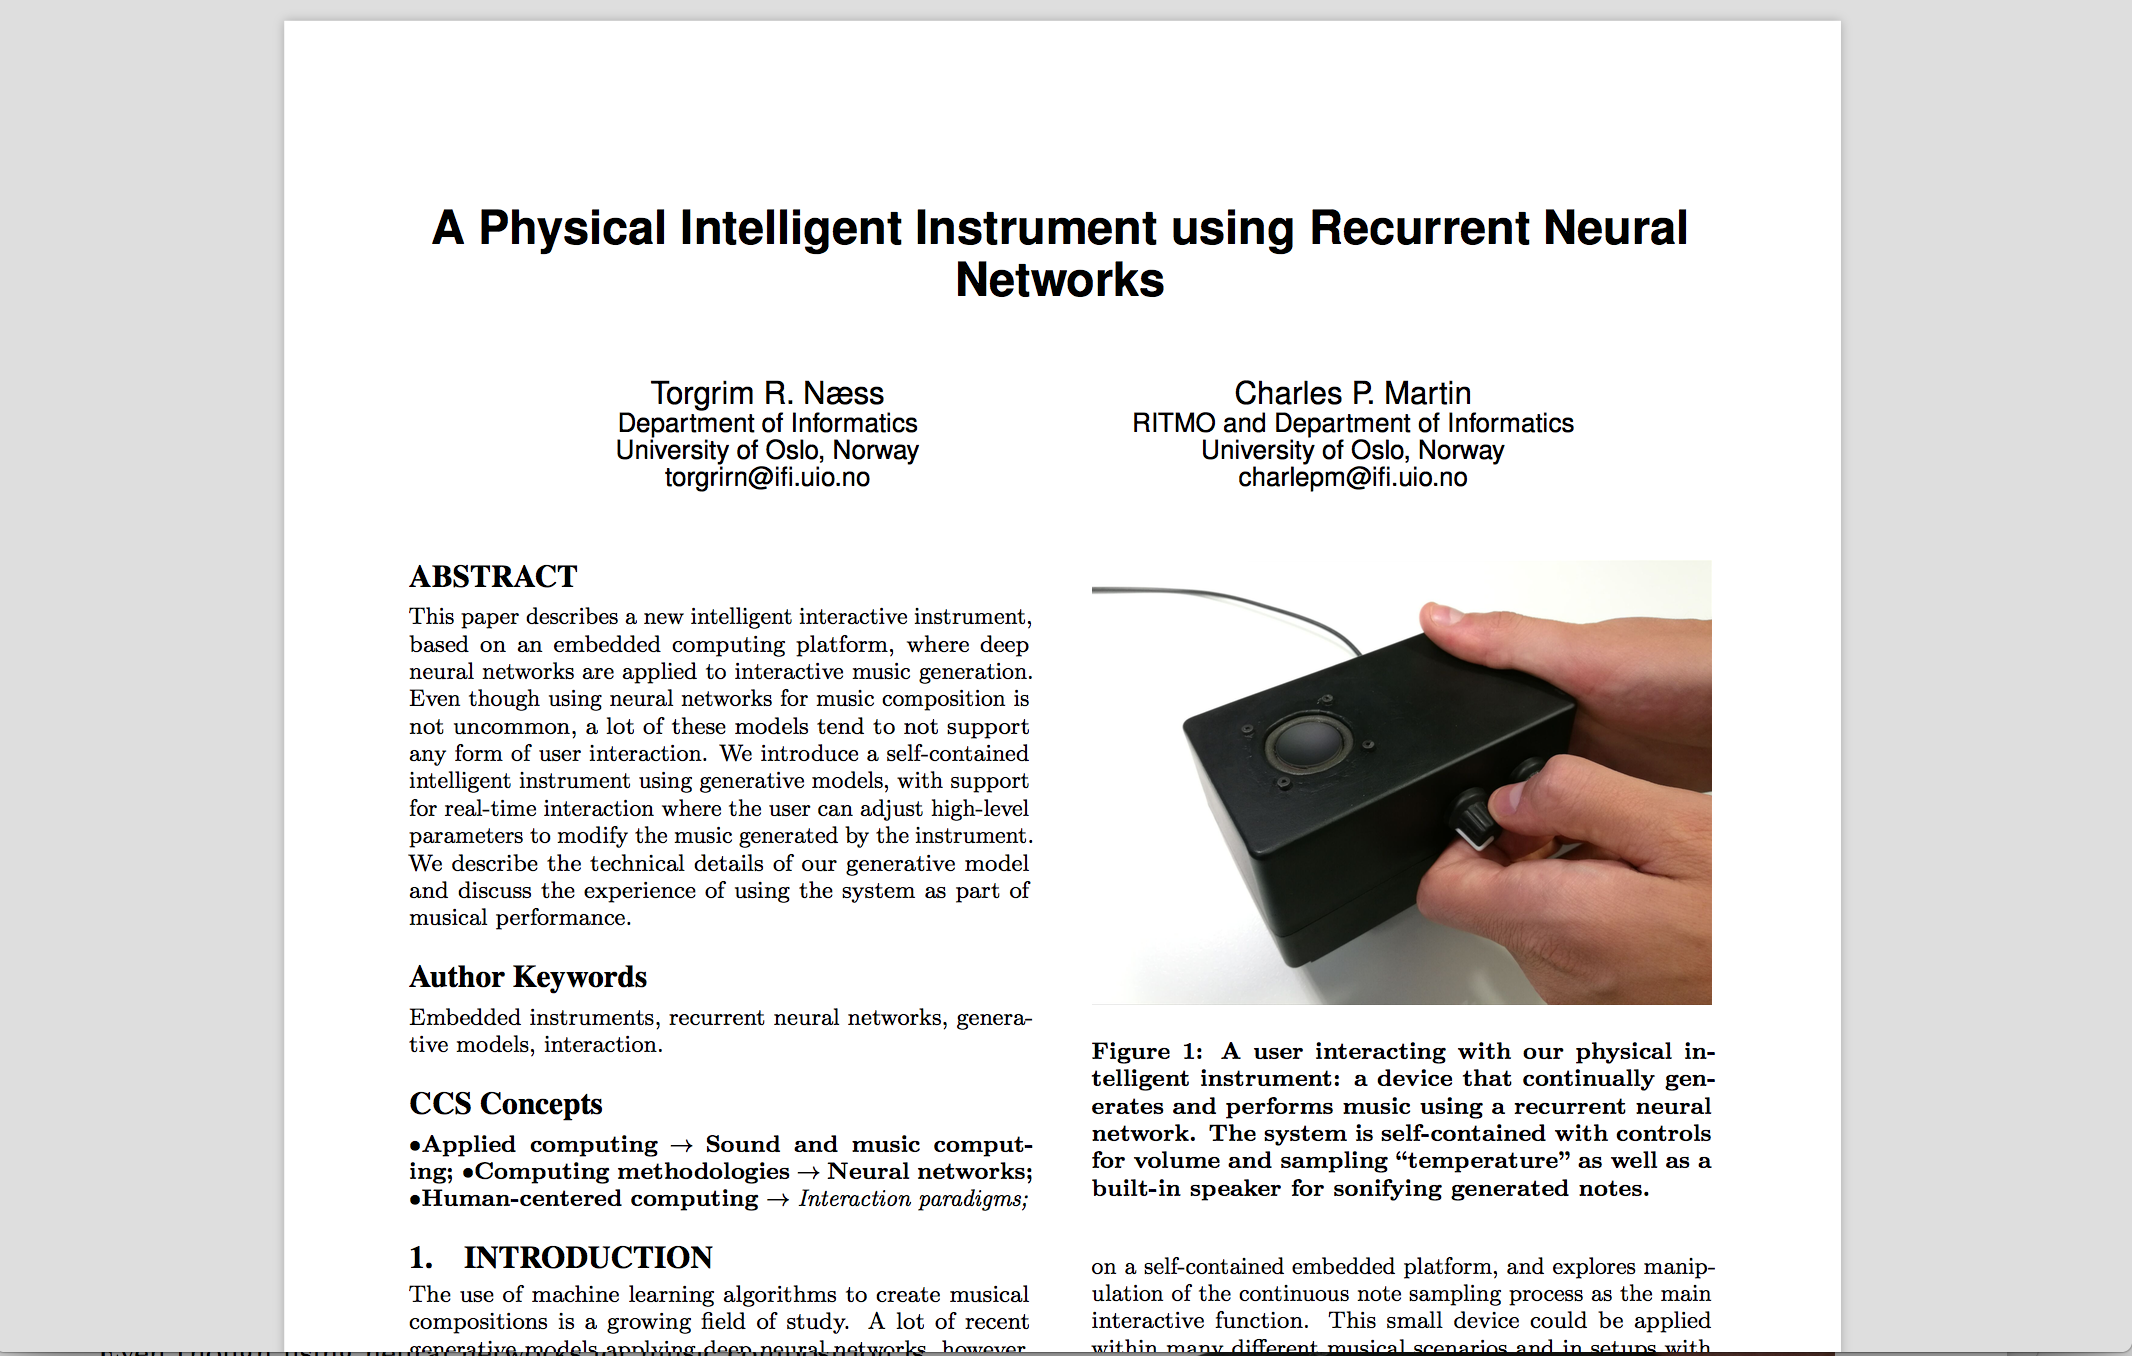
\includegraphics[scale=0.31]{img/Torgrim-NIME-2019.png}\\
	    \cite{Naess.2019.NIME}\\
	       {\scriptsize  \url{https://github.com/edrukar/intelligent_instrument}}
   \end{figure}	
\end{frame}
%
\begin{frame}
\frametitle{}
 \begin{figure}
	
\includegraphics[scale=0.3]{img/Torgrim-masterthesis-2019.png}
    \end{figure}		
\end{frame}
%
\begin{frame}
\frametitle{A Physical Intelligent Instrument}	
\begin{itemize}
\item RQ: Exploration of whether intelligent musical systems can provide an easier introduction into music creation for novice users focusing on a self-contained intelligent instrument using generative models.
\item Evaluation:
\begin{itemize}
\item User study with 12 participants.
\item (1) impact the different high-level parameter controls on participant's perception of musical instrument's control and (2) Evaluation of the generative models trained on different datasets in terms of musical quality.
\item Collected numerical ratings and open-ended answers (mixed methods).
\end{itemize}
\item Results: Perceived feeling of control over the music was quite high and the high- level parameter controls allowed participants to creatively engage with the instrument in the music-making process.
\item Contribution: Informs DMIs design \& evaluation using machine learning and embedded computing.
\end{itemize}
\end{frame}
%
\begin{frame}
\frametitle{}
 \begin{figure}
	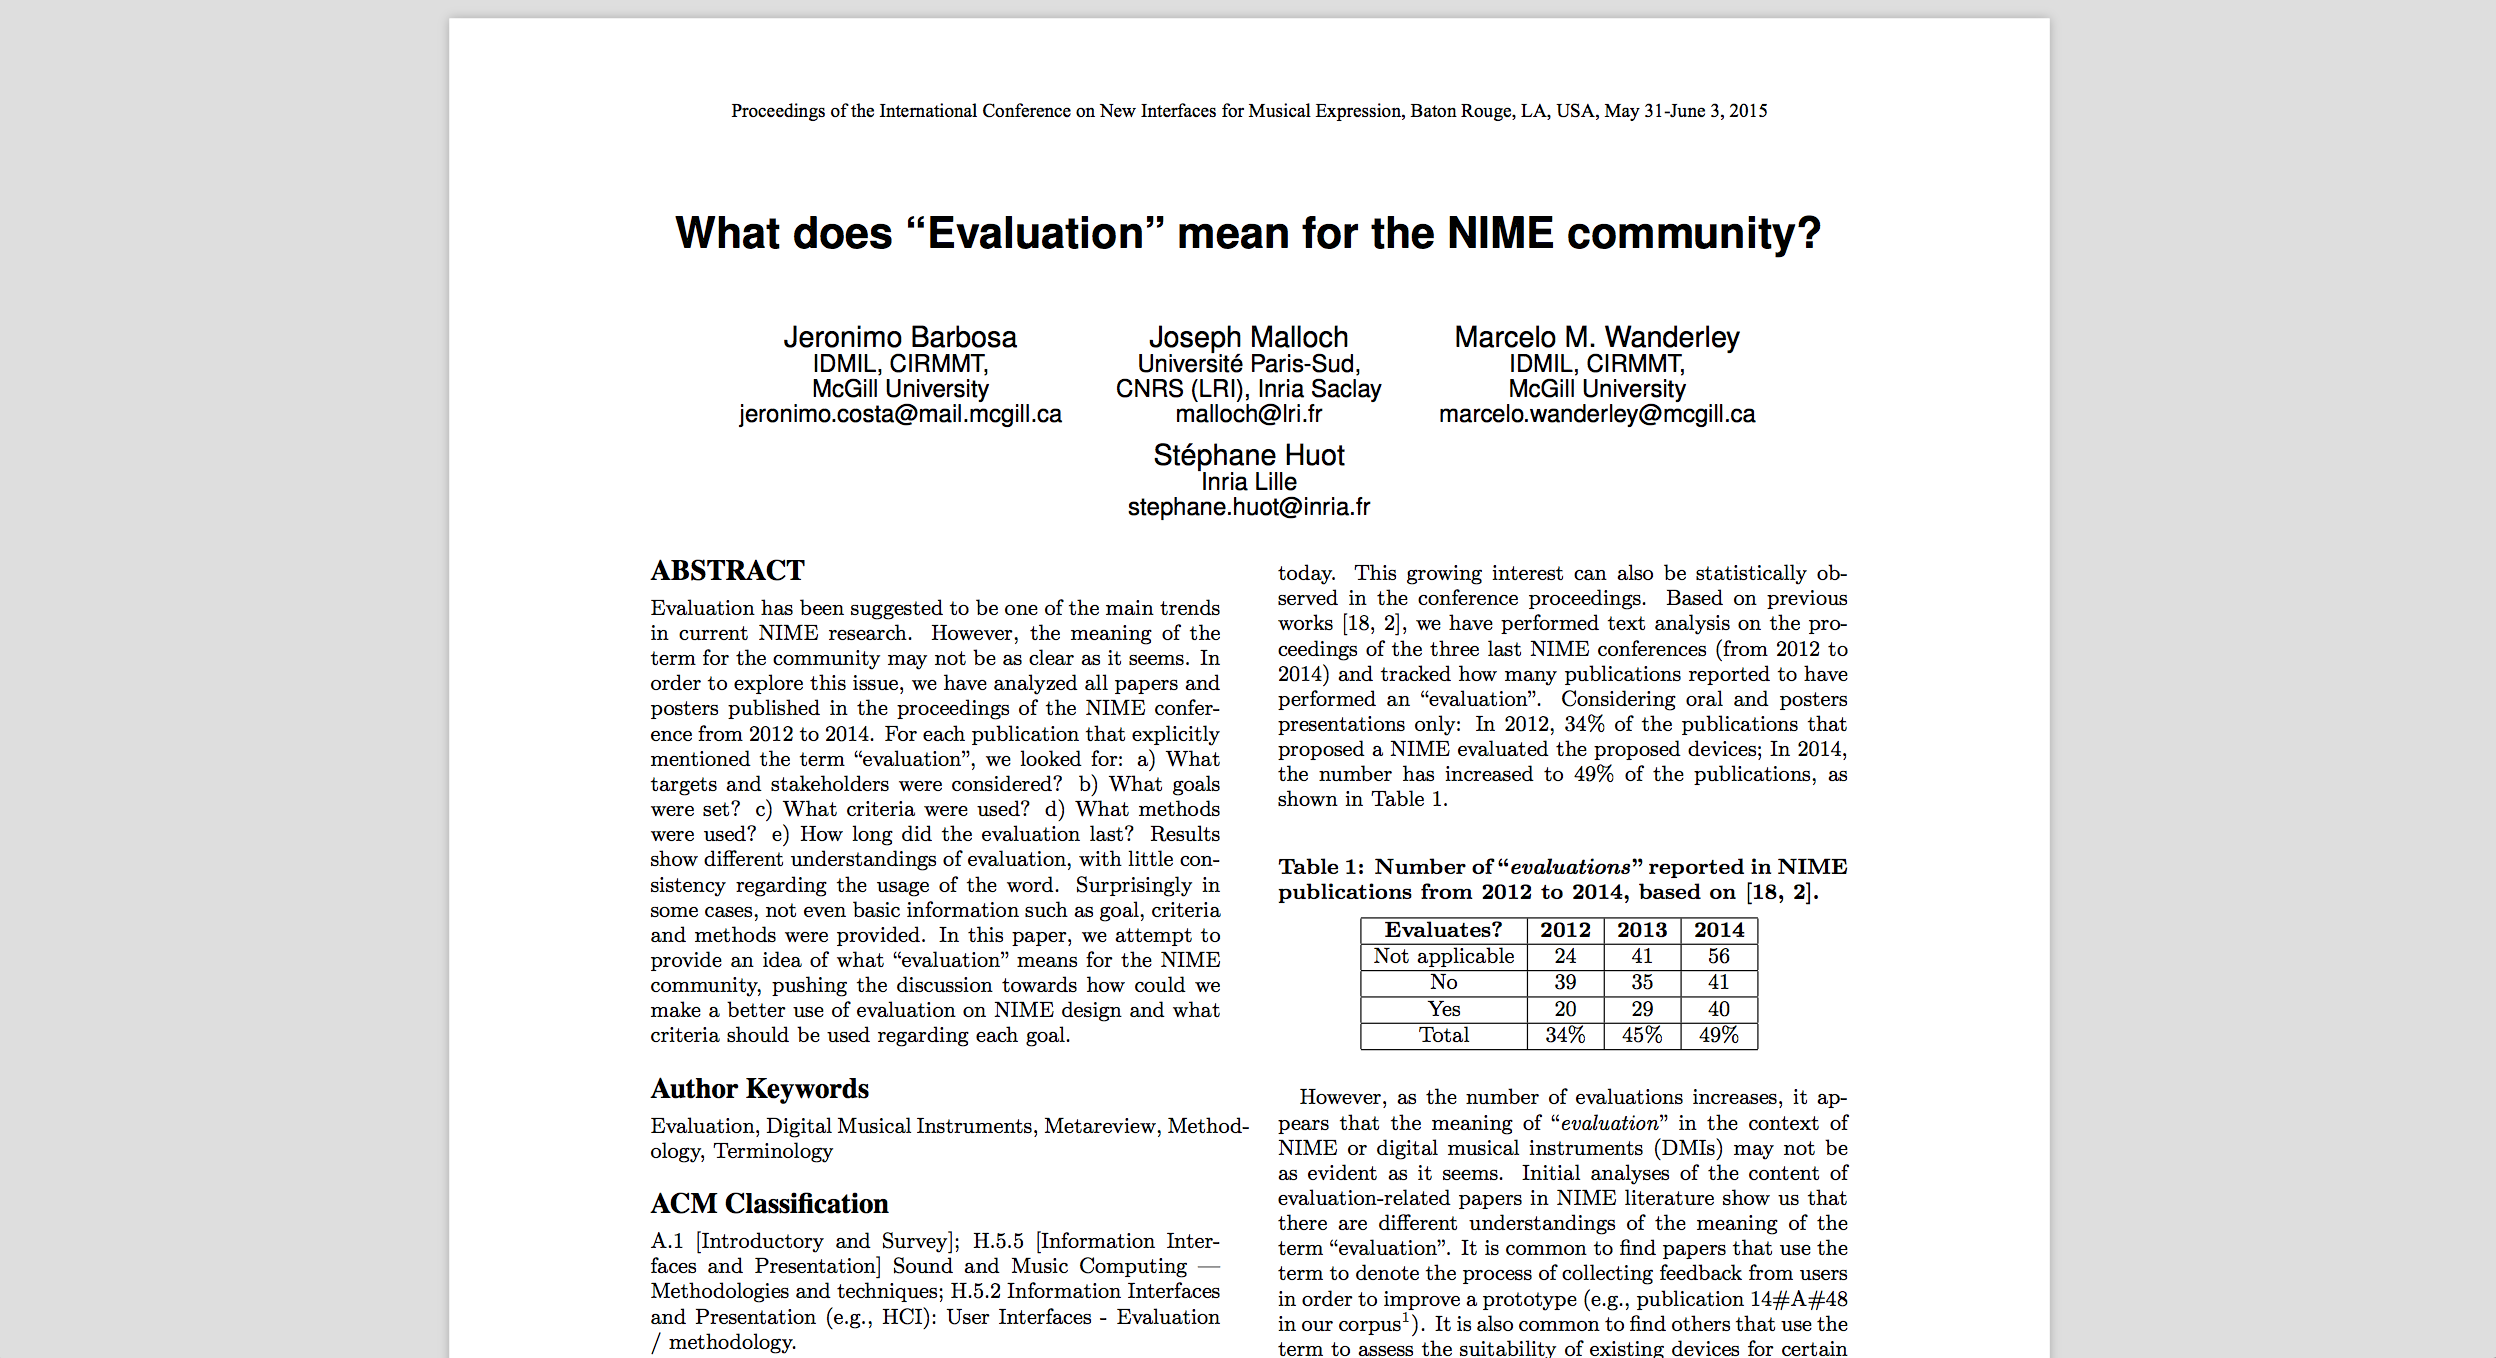
\includegraphics[scale=0.25]{img/Barbosa-et-al-2015.png}
    \end{figure}	
\begin{quote}There is no one-size-fits-all solution to evaluating DMIs and more precisely the choice of evaluation methodology -- if any -- must arise from and be appropriate for the actual problem or research question under consideration. \cite[p.161]{Barbosa.et.al.2015.evaluationNIME}
\end{quote}
\end{frame}


%
%\begin{frame}
%\frametitle{Preparation: Mindmap}
%\begin{itemize}
%\item Create an intuitive mindmap based on a brainstorming session with your team about the topics from NIME and HCI that you think are related to the prototype that you built during the physical computing workshop.
%\end{itemize}
%\end{frame}
%
%\begin{frame}
%\frametitle{Mapping the NIME field}
%\begin{itemize}
%\item Presentations and discussion about the mindmaps:
%\begin{itemize}
%\item What was the workflow to create the mindmap? (e.g. from paper to digital, Chinese whispers styles, etc)
%\item What tool(s) have you used?
%\item How did you come across with the concepts?
%\end{itemize}
%\end{itemize}
%\end{frame}
%%
%\begin{frame}
%\frametitle{Presentation/lecture: NIME (practices)}
%\begin{itemize}
%\item Presentation/lecture of a selection of practices in NIME from an HCI perspective + Q\&A.
%\end{itemize}
%\end{frame}

%
\begin{frame}
\frametitle{}
\Huge{NIME Paper Writing}
\end{frame}
%
\begin{frame}
\frametitle{Teamwork: Understanding NIME paper writing}
\begin{itemize}
\item Selection of a paper from the NIME Reader (\url{https://www.springer.com/gp/book/9783319472133}), PDFs can be found in NIME Proceedings (\url{http://www.nime.org/archives/}).
Discussion about what is ... 
\begin{itemize}
\item the research question (RQ)
\item the approach used to address the RQ / research methods
\item the main findings 
\item the main contribution
\end{itemize}
A high-level summary comparison between the format of NIME and CHI papers is acknowledged.
\end{itemize}
\end{frame}
%
\begin{frame}
\frametitle{Teamwork: Summaries}
\begin{itemize}
\item The teams summarize to the group their selected paper (10 min per group). 
\begin{itemize}
\item research question (RQ)
\item approach to address the RQ / research methods
\item main findings 
\item main contribution
\end{itemize}
\item Comparison with CHI papers: what are the similarities and differences? 
\end{itemize}
\end{frame}
%
\begin{frame}
\frametitle{Human-Computer Interaction Day 3 - Group Assignment (post-class)}
\begin{itemize}
\item Create an intuitive mindmap based on a brainstorming session with your team about the topics from NIME and HCI that you think are related to the prototype that you built during the physical computing workshop. This assignment (a digital version of the mindmap) should be submitted before Thursday 31 October 2019 9:00 and the team should be ready to briefly summarize it in class.
\end{itemize}
\url{https://uio.instructure.com/courses/22318/assignments/28317}
\end{frame}
%
%\begin{frame}
%\frametitle{Resources}
%\begin{itemize}
%\item The content of this class can be found on Canvas here:\\
%\url{https://uio.instructure.com/courses/11472/pages/human-computer-interaction-2a}
%\item The slides of this class can be found on GitHub here: \\
%\url{https://github.com/axambo/hci-lecture-slides/tree/master/slides/d3/}
%\item Archive of NIME Proceedings:\\
%\url{http://www.nime.org/archives/}
%\end{itemize}
%\end{frame}
%
\begin{frame}[shrink=20]
  \frametitle{References}
  \printbibliography
\end{frame}
%
\end{document}
